%
% $RCSfile$
%
% Copyright (c) 2005-2006. Christian Heller. All rights reserved.
%
% Permission is granted to copy, distribute and/or modify this document
% under the terms of the GNU Free Documentation License, Version 1.1 or
% any later version published by the Free Software Foundation; with no
% Invariant Sections, with no Front-Cover Texts and with no Back-Cover
% Texts. A copy of the license is included in the section entitled
% "GNU Free Documentation License".
%
% http://www.cybop.net
% - Cybernetics Oriented Programming -
%
% http://www.resmedicinae.org
% - Information in Medicine -
%
% Version: $Revision$ $Date$ $Author$
% Authors: Christian Heller <christian.heller@tuxtax.de>
%

\subsection{Knowledge Schema}
\label{knowledge_schema_heading}

Human beings have a brain which they use to think, in other words to build up a
mind. While the former exists in the \emph{Real World}, the latter is
constructed as a subjective \emph{Virtual World}. All people do think, all the
time, even not knowing that they do. One would therefore guess that the act of
\emph{Thinking} is a most common one, familiar to anybody. But judging from the
enormous research effort in sciences dealing with it, the \emph{Principles}
behind thinking are not that easy to grasp.

%
% $RCSfile: schema.tex,v $
%
% Copyright (c) 2005-2006. Christian Heller. All rights reserved.
%
% Permission is granted to copy, distribute and/or modify this document
% under the terms of the GNU Free Documentation License, Version 1.1 or
% any later version published by the Free Software Foundation; with no
% Invariant Sections, with no Front-Cover Texts and with no Back-Cover
% Texts. A copy of the license is included in the section entitled
% "GNU Free Documentation License".
%
% http://www.cybop.net
% - Cybernetics Oriented Programming -
%
% http://www.resmedicinae.org
% - Information in Medicine -
%
% Version: $Revision: 1.1 $ $Date: 2006-01-03 08:21:45 $ $Author: christian $
% Authors: Christian Heller <christian.heller@tuxtax.de>
%

\subsubsection{Schema}
\label{schema_heading}

A theoretical \emph{Model} is an abstract clip of the real world, and exists in
the human mind. Another common word for \emph{Model} is \emph{Concept}. It is
the subsumption of \emph{Item}, \emph{Category} and \emph{Compound}, resulting
from three activities of abstraction: \emph{Discrimination},
\emph{Categorisation} and \emph{Composition} \cite{heller2004}. Each model
\emph{knows} about the parts it consists of.

\begin{figure}[ht]
    \begin{center}
        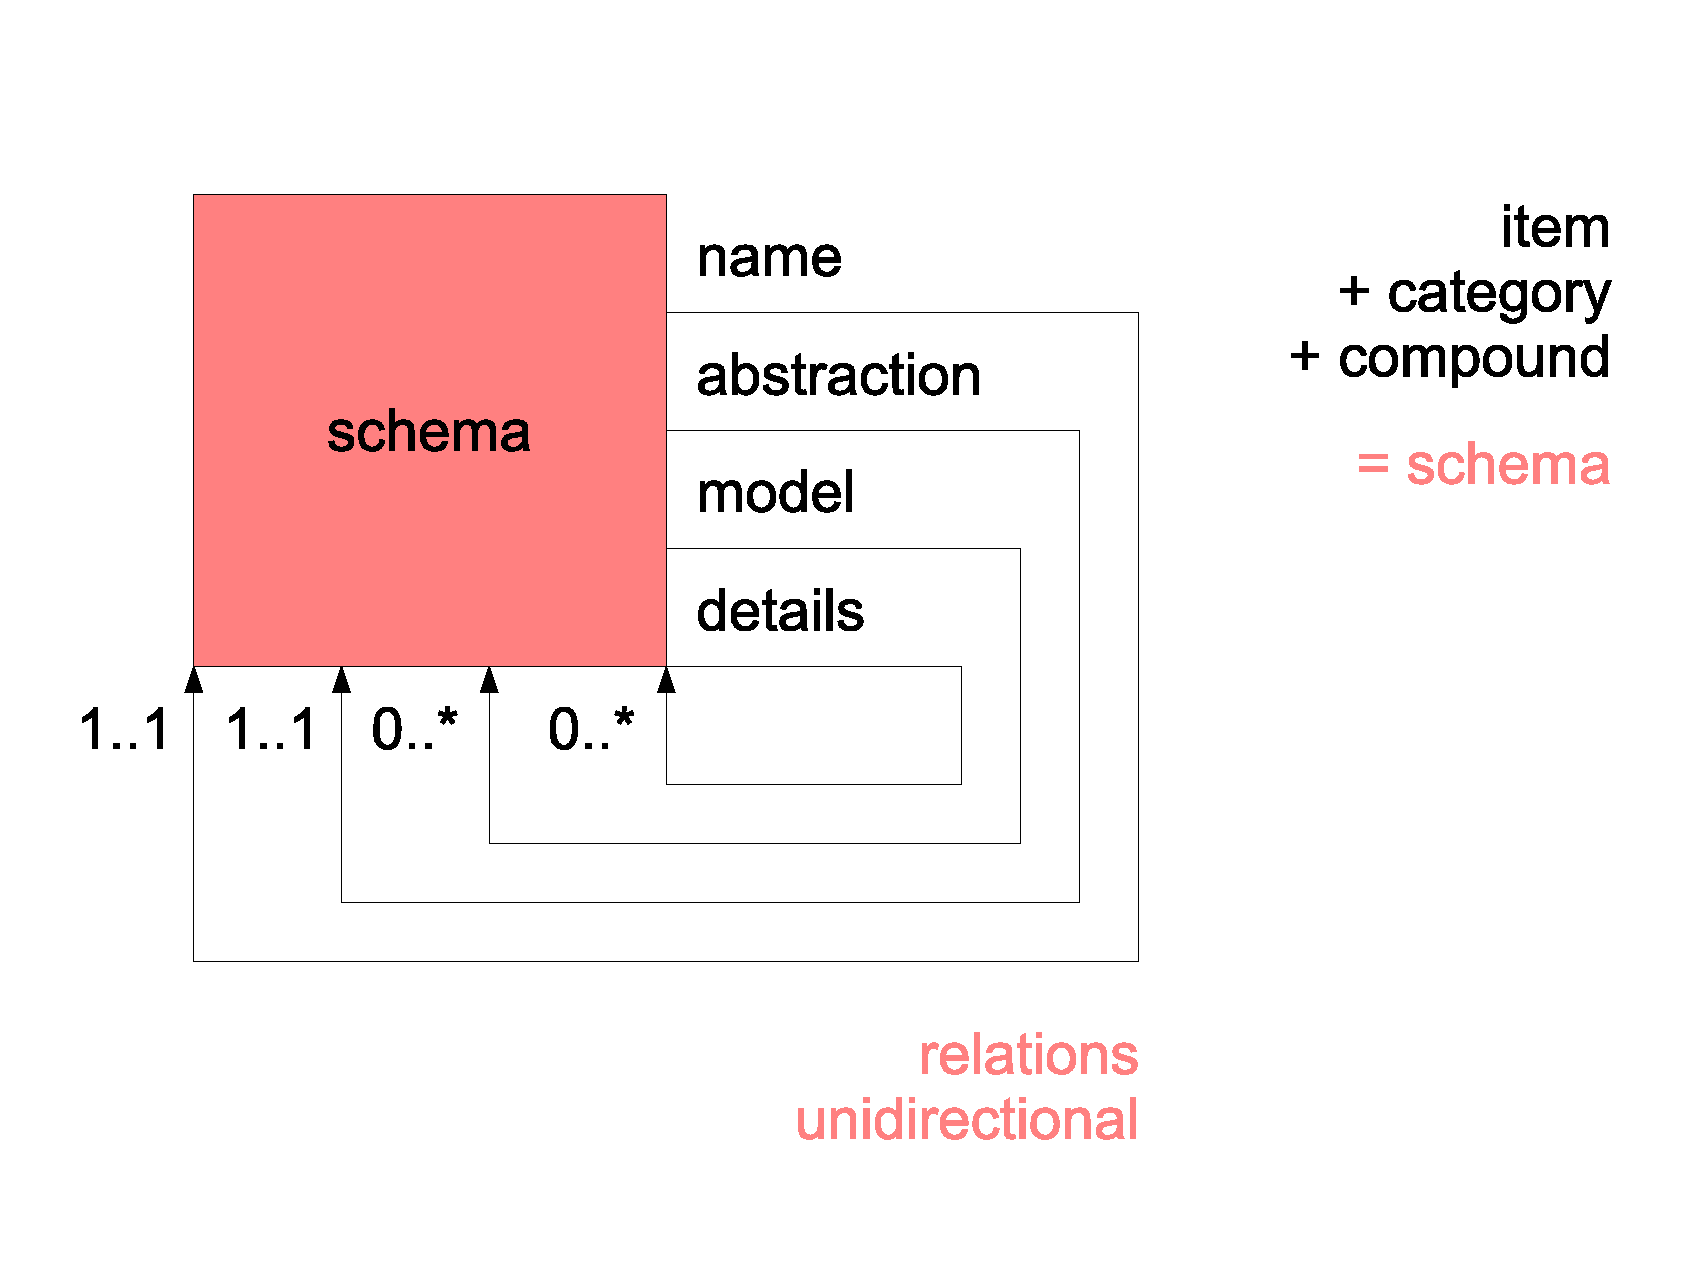
\includegraphics[scale=0.2]{vector/schema.eps}
        \caption{Knowledge Schema}
        \label{schema_figure}
    \end{center}
\end{figure}

Yet what does this knowledge of a compound model (whole) about its parts imply?
Software developers call knowledge \emph{about} something
\emph{Meta Information}. Figure \ref{schema_figure} illustrates a
\emph{Schema} (structure) with four kinds of meta information in a whole-part
relation.

An obvious way is to give each part a unique \emph{Name} for identification.
Secondly, a compound needs to know about the \emph{Model} of each part since a
part may itself be seen as compound that needs to know about its parts. The
distinction of the several kinds of models, in other words the kind of
\emph{Abstraction} (compound, term, number etc.) of a model is the third kind
of information a compound needs to know about its parts. It is comparable to a
\emph{Type} in classical system programming languages. All further kinds of
meta information are summed up by a fourth relation which is called
\emph{Details}.

%
% $RCSfile: double_hierarchy.tex,v $
%
% Copyright (C) 2002-2008. Christian Heller.
%
% Permission is granted to copy, distribute and/or modify this document
% under the terms of the GNU Free Documentation License, Version 1.1 or
% any later version published by the Free Software Foundation; with no
% Invariant Sections, with no Front-Cover Texts and with no Back-Cover
% Texts. A copy of the license is included in the section entitled
% "GNU Free Documentation License".
%
% http://www.cybop.net
% - Cybernetics Oriented Programming -
%
% http://www.resmedicinae.org
% - Information in Medicine -
%
% Version: $Revision: 1.1 $ $Date: 2008-08-19 20:41:06 $ $Author: christian $
% Authors: Christian Heller <christian.heller@tuxtax.de>
%

\subsection{Double Hierarchy}
\label{double_hierarchy_heading}
\index{Double Hierarchy}
\index{Whole-Part Relationship}
\index{Dialectical Relationship between Whole and Part}
\index{Conceptual Interaction}
\index{Part}
\index{Property}
\index{Constraint}

Finally, what makes up the character of a model (in the understanding of the
human mind) is a combination of two hierarchies: the \emph{Parts} it consists
of, together with \emph{Meta Information} about it.

Most properties of a molecule in \emph{Chemistry}, for example, are determined
by the number and arrangement of its atoms. \emph{Hydrogen} (H$_{2}$) becomes
\emph{Water} (H$_{2}$O) (with a totally different character) when just one
\emph{Oxygen} (O) atom is added per hydrogen molecule. The Wikipedia Encyclopedia
\cite{wikipedia} cites and writes about Richard Levins and Richard Lewontin
who, in their book \textit{The Dialectical Biologist} \cite{levins}, sketch a
\emph{dialectical} approach to biology:

\begin{quote}
    They focus on the (dialectical) relationship between the \emph{Whole} (or
    \emph{Totality}) and the \emph{Parts}: \textit{Part makes Whole, and Whole
    makes Part} \cite[p. 272]{levins}. That is, a biological system of some kind
    consists of a collection of heterogeneous parts. All of these contribute to
    the character of the whole, as in reductionist thinking. On the other hand,
    the whole has an existence independent of the parts and feeds back to affect
    and determine the nature of the parts. This back-and-forth (dialectic) of
    causation implies a dynamic process. \ldots\ Further, each species is part
    of the \emph{Environment} of all of the others.
\end{quote}

The kinds of meta information discussed in the previous sections were also
called \emph{Dimensions} or \emph{Conceptual Interaction} between a \emph{Whole}
and its \emph{Parts}. They may represent very different properties and each of
them may be constrained to certain values- or areas of validity.

\begin{figure}[ht]
    \begin{center}
        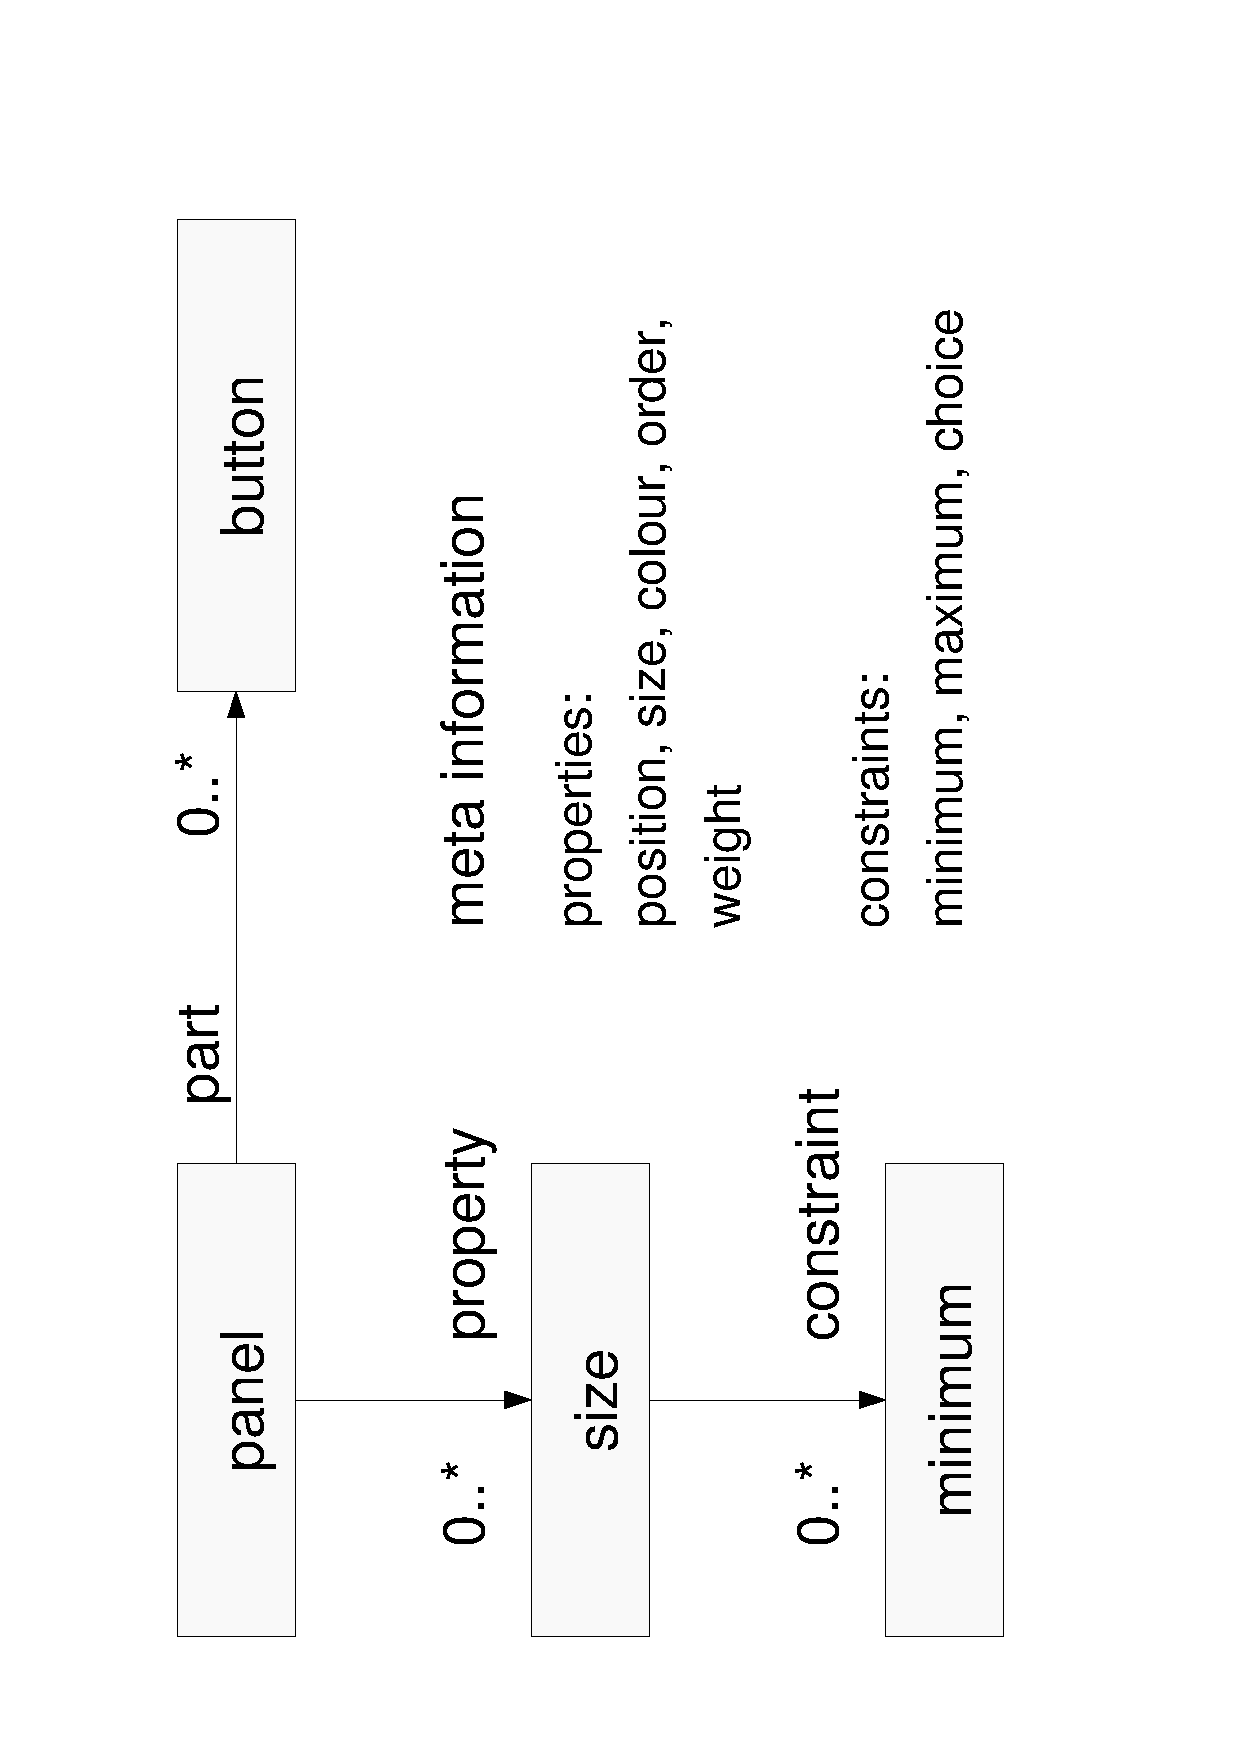
\includegraphics[scale=0.3,angle=-90]{graphic/double.pdf}
        \caption{Double Hierarchy of Parts and Meta Information}
        \label{double_figure}
    \end{center}
\end{figure}

Figure \ref{double_figure} illustrates the \emph{Double Hierarchy} here
spoken of. A graphical panel was chosen as example model. It may consist of
smaller parts, among them being a number of buttons. Altogether, they form the
\emph{Part Hierarchy}. On the other hand, there are properties like the size,
position or colour of the buttons, which are neither part of the panel, nor of
the buttons themselves; they are information \emph{about} the buttons and form
an own \emph{Meta Hierarchy}. To the latter do also belong constraints like the
minimum size of a button or a possible choice of colours for it. Constraints can
be treated like meta information about properties. Once again: \emph{Properties}
are information about a \emph{Part}; \emph{Constraints} are information about a
\emph{Property}.

%
% $RCSfile$
%
% Copyright (c) 2002-2006. Christian Heller. All rights reserved.
%
% Permission is granted to copy, distribute and/or modify this document
% under the terms of the GNU Free Documentation License, Version 1.1 or
% any later version published by the Free Software Foundation; with no
% Invariant Sections, with no Front-Cover Texts and with no Back-Cover
% Texts. A copy of the license is included in the section entitled
% "GNU Free Documentation License".
%
% http://www.cybop.net
% - Cybernetics Oriented Programming -
%
% http://www.resmedicinae.org
% - Information in Medicine -
%
% Version: $Revision$ $Date$ $Author$
% Authors: Christian Heller <christian.heller@tuxtax.de>
%

\subsubsection{Container Unification}
\label{container_unification_heading}

Section \ref{motivation_heading} mentioned container inheritance as one problem
of current software. Due to polymorphism, it may cause unpredictable behaviour
possibly leading to \emph{falsified} container contents \cite{javaiaq}. The
previous sections introduced a knowledge schema which they claimed to be
\emph{general}. But that also means that all kinds of containers must be
representable by the suggested schema. But why are there so many different
kinds of containers? What actually is a container?

It is a concept expressing that some model \emph{contains} some other model(s).
Types of containers are, for example: \emph{Collections} (Array, Vector, Stack,
Set, List), \emph{Maps} (Hash Map, Hash Table) and the \emph{Tree}. They all
are containers. What differs, is just the meta information they store about
their elements. A list, for example, holds position information about each of
its elements. A map relates the name of an element to its model (1:1). A tree
links one model to many others (1:n).

But does the different meta information a container holds about its elements
justify the existence of different container models? If a knowledge schema was
general enough to represent a container structure on one hand, and to express
different kinds of meta information on the other, it might be able to behave
like any of the known container types.

The schema proposed in this work claims to be this kind of knowledge schema. It
has a container structure by default, and can thus hold many parts in a
\emph{Tree}-like manner. It holds standard meta information about its parts:
their \emph{Name}, \emph{Model}, kind of \emph{Abstraction} and further meta
information called \emph{Details} -- and is therefore able to link the name of
an element to its model, in a \emph{Map}-like manner. To the additional meta
information (details) may belong the \emph{Position} of an element within its
model, in a \emph{List}-like manner. A \emph{Table} structure can be represented
as well, by splitting it into a hierarchical (tree-like) representation, as
known from markup languages like the \emph{Hypertext Markup Language} (HTML).

Section \ref{cybol_heading} will introduce a language capable of expressing all
aspects of the knowledge schema as proposed here.

%
% $RCSfile: universal_memory_structure.tex,v $
%
% Copyright (C) 2002-2008. Christian Heller.
%
% Permission is granted to copy, distribute and/or modify this document
% under the terms of the GNU Free Documentation License, Version 1.1 or
% any later version published by the Free Software Foundation; with no
% Invariant Sections, with no Front-Cover Texts and with no Back-Cover
% Texts. A copy of the license is included in the section entitled
% "GNU Free Documentation License".
%
% http://www.cybop.net
% - Cybernetics Oriented Programming -
%
% http://www.resmedicinae.org
% - Information in Medicine -
%
% Version: $Revision: 1.1 $ $Date: 2008-08-19 20:41:09 $ $Author: christian $
% Authors: Christian Heller <christian.heller@tuxtax.de>
%

\subsection{Universal Memory Structure}
\label{universal_memory_structure_heading}
\index{Universal Memory Structure}
\index{Structured- and Procedural Programming}
\index{SPP}
\index{Object Oriented Programming}
\index{OOP}
\index{Design Time Structure}
\index{Runtime Structure}
\index{Knowledge Schema}

To better explain the differences between traditional- and cybernetics-oriented
design models, a further example shall be given. Figure \ref{universal_figure}
illustrates design-time structures in the upper half, and runtime structures in
the lower. Using \emph{Structured- and Procedural Programming} (SPP) or
\emph{Object Oriented Programming} (OOP), a developer would design a model as
shown on the upper left-hand side in the figure. (The fact that OOP also offers
inheritance relations and OOP classes do own methods in addition to attributes,
while SPP structures do not, is of minor importance here.) At runtime, exactly
that model would be applied to structure instances and their relations
accordingly, as shown on the lower left-hand side in the figure.

\begin{figure}[ht]
    \begin{center}
        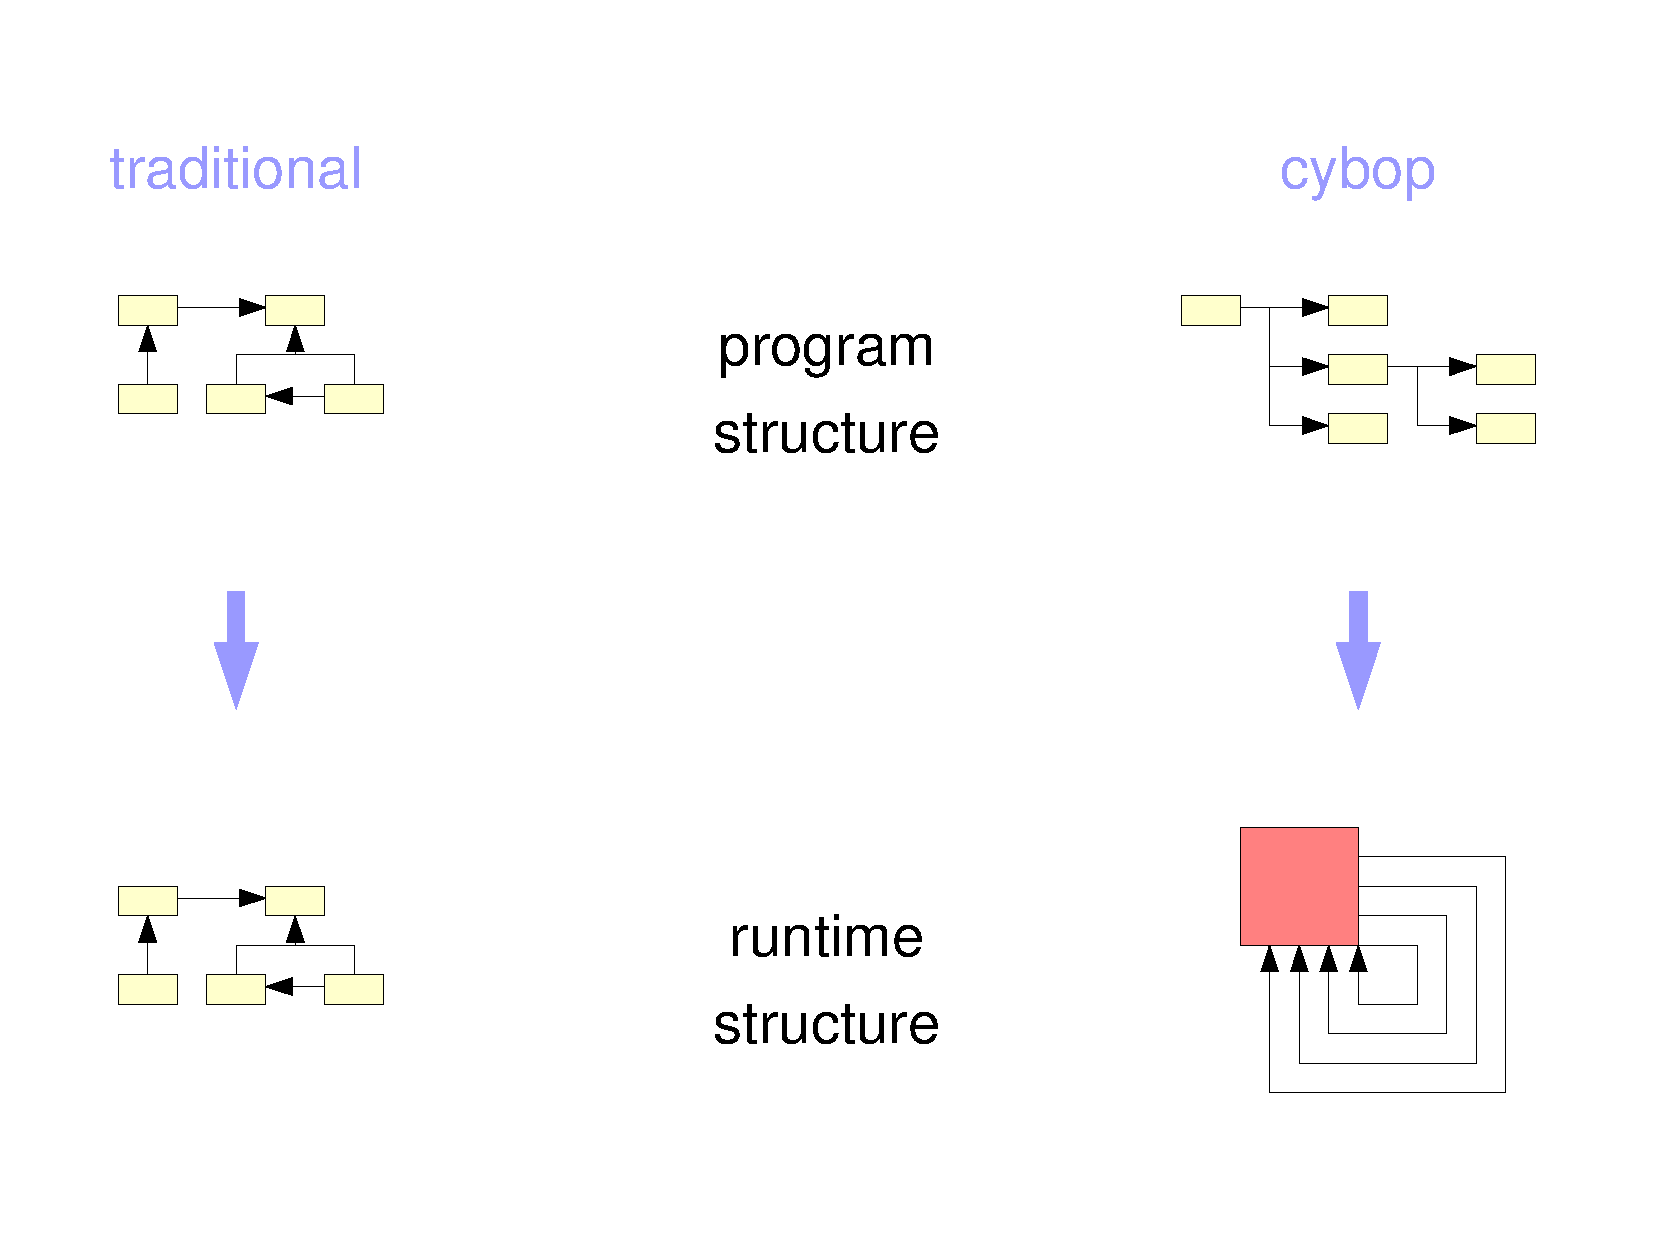
\includegraphics[scale=0.3,angle=-90]{graphic/universal.pdf}
        \caption{Universal Memory Structure}
        \label{universal_figure}
    \end{center}
\end{figure}

Not so in \emph{Cybernetics Oriented Programming} (CYBOP). Knowledge templates
as created at design time do always have a hierarchical structure, as shown on
the upper right-hand side in the figure. They include \emph{Whole-Part-} as
well as \emph{Meta Hierarchies}. At runtime, these templates get cloned by
creating models that follow the structure of the CYBOP \emph{Knowledge Schema},
as shown on the lower right-hand side in the figure. While SPP/ OOP rely on a
variety of different structures to store knowledge in memory, CYBOP uses one
\emph{Universal Memory Structure} (knowledge schema) that, so to say, merges
traditional structures like different kinds of \emph{Containers}, \emph{Class}
and \emph{Record}/\emph{Struct}. Even algorithmic structures (logic)
traditionally stored in a \emph{Procedure} are covered by this knowledge
schema. More on state and logic in the following chapter.

The advantages are obvious. Data available in a unified structure are easier to
process. Dependencies of the knowledge schema are defined clearly and remain
the same for all applications, so that domain/ application knowledge becomes
independent from the underlying system control software. Global data access and
bidirectional dependencies are not necessary anymore, since every knowledge
model can be accessed along well-defined paths within the knowledge hierarchy.
Byte code manipulation and similar tricks and workarounds might finally belong
to the past.

